\section{Hard sync 的有限词表数值核验}
\label{sec:hard-sync-experiments}

本节用完全可求解的 categorical 子问题核验前述动力学。实验程序为 \path{experiments/toy/hard_sync_audit.py}，结果保存在 \path{results/hard-sync-audit/}。所有计算使用 float64，随机种子为 $20261010$。这是固定 prefix 下的分布空间实验；其证据范围是精确更新与受控输出扰动，LLM 的参数共享、随机梯度和 rollout 变化需要分别测量。

\subsection{实验问题与可证伪的判据}

实验在运行前固定以下判据。
\begin{enumerate}
 \item Gibbs 的跨度递推与三点 KL 恒等式应在数值误差内成立。词表大小取 $2,4,8$，每个大小生成 $12$ 组独立正分布，步长取 $0.2,0.8,1,1.2,1.8,2,2.2$，共检查 $252$ 个更新。绝对残差阈值取 $10^{-12}$。
 \item 独立 SciPy Lambert-$W$ 求解器与仓库 \path{token_inner.mean_target} 的 $36$ 组输出逐坐标差不超过 $10^{-12}$。各步长的 Mean KKT 残差与归一化残差也不超过 $10^{-12}$。这同时检查理论更新与参考实现的对应关系。
 \item 固定 $t=(0.2,0.3,0.5)$、$z=(-1,0.2,0.8)$，令 $q_\epsilon\propto t\exp(\epsilon z)$。扫描 $\epsilon=0.4,0.2,0.1,0.05,0.02,0.01$，Mean 在 $\eta=1$ 时的 KL 三次比值应趋于一；最小 $\epsilon$ 的相对偏差阈值为 $2\%$。
 \item 同一 teacher 下，从 $q_0\propto t\exp(0.2z)$ 出发，运行 $\eta=2$ 的 $10000$ 轮精确更新。Gibbs 应保持二周期，Mean 的 $k\KL(\pi_k\Vert t)$ 应接近 $1/16$；最终绝对偏差阈值为 $0.004$。
 \item 输出噪声和 reward 噪声分别按式~\eqref{eq:hs-centered-linear} 注入。用 $20000$ 条独立路径、$240$ 步以及 $\eta=0.2,0.5,1,1.5,1.8$，比较 teacher 加权二阶矩的样本均值和精确有限时间预测。每个均值须落在预测值的五个 Monte Carlo 标准误差以内。
\end{enumerate}

\subsection{数值稳定性与局部阶数}

KL 三次收敛会迅速产生接近机器精度的 KL。直接计算 $\sum_a p_a\log(p_a/t_a)$ 会把一阶正负项相消，影响三次比值。令 $d_a=p_a/t_a-1$，归一化给出 $\sum_a t_ad_a=0$，因此改写为
\[
 \KL(p\Vert t)=\sum_a t_a\{(1+d_a)\log(1+d_a)-d_a\}.
\]
当 $|d_a|<10^{-3}$ 时，程序使用
\[
 (1+d)\log(1+d)-d
 =\sum_{n=2}^{9}\frac{(-1)^n d^n}{n(n-1)}+O(d^{10}).
\]
这保留局部 KL 的二阶首项。Mean 归一化根也用 $\E_q\operatorname{expm1}(G-W_0(\lambda e^G))=0$ 求解，避免两个接近一的数相减。求根器同时记录 KKT 残差。

本方向的 teacher 方差与跨度为
\[
 \Var_t(z)=0.4644,\qquad \operatorname{osc}z=1.8,
\]
所以理论预测
\[
 \frac{b(p^\star,t)}{b(q_\epsilon,t)^3}\to
 \frac{0.4644}{2\cdot1.8^2}=0.071666\ldots.
\]
逐点数值与 KL 三次比值保存在 \path{cubic.csv}；它们检验乘子的二阶修正，而非仅检验一次线性化。

预设的各项数值判据均通过。表~\ref{tab:hard-sync-audit} 汇总残差与局部、边界常数；这里的实测值来自上述固定配置。
\begin{table}[htbp]
 \centering
 \caption{精确 hard-sync 更新的数值核验。}
 \label{tab:hard-sync-audit}
 \begin{tabular}{ll}
 \toprule
 项目 & 实测结果\\
 \midrule
 Gibbs 三点恒等式最大绝对残差 & $1.78\times10^{-15}$\\
 Mean 独立求解与参考实现最大坐标差 & $2.78\times10^{-16}$\\
 Mean KKT 与归一化最大残差 & $3.55\times10^{-15}$\\
 $\epsilon=0.01$ 的 KL 三次比值 & $1.011557$，极限为 $1$\\
 同一点的跨度三次比值 & $0.071591$，极限为 $0.071667$\\
 $\eta=2$、$k=10000$ 的 Mean $k\KL$ & $0.062303$，极限为 $0.0625$\\
 \bottomrule
 \end{tabular}
\end{table}

\subsection{边界阻尼与噪声位置}

图~\ref{fig:hard-sync-audit} 左侧比较同一初值下的边界步长：Gibbs 的两周期与 Mean 的缓慢衰减清楚分离。虚线是独立推导的 $1/(16k)$，并未用实验数据拟合。

右侧从零误差出发，先生成独立 $N(0,\sigma^2I)$ 向量，再减去其 teacher 均值，取 $\sigma=0.01$。该居中噪声满足
\[
 \E\|\xi\|_t^2=\sigma^2\left(1-\sum_a t_a^2\right).
\]
对固定输出噪声，有限时间精确预测为
\[
 \E\|y_K\|_t^2=
 \sigma^2\left(1-\sum_a t_a^2\right)
 \frac{1-(1-\eta)^{2K}}{\eta(2-\eta)}.
\]
对于 reward 噪声，再乘 $\eta^2$。图中误差条是均值的 $1.96$ 个标准误差，虚线是上述预测。两个噪声模型呈现不同步长趋势，与输入位置的理论分析一致。

\begin{figure}[htbp]
 \centering
 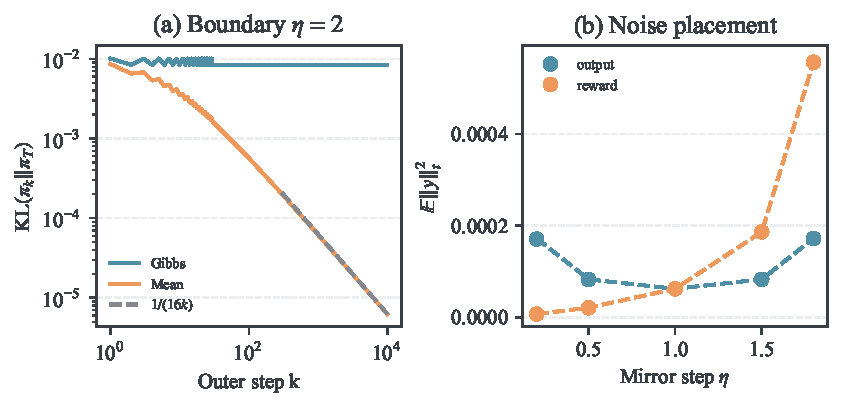
\includegraphics[width=0.96\textwidth]{../../results/hard-sync-audit/hard-sync.pdf}
 \caption{固定三元词表下的 hard-sync 审计。左：$\eta=2$ 的精确 Gibbs 与 Mean teacher KL；右：固定输出噪声和固定 reward 噪声的 teacher 加权二阶矩。点和实线来自数值更新，虚线来自独立理论预测。}
 \label{fig:hard-sync-audit}
\end{figure}

实验中的浮点求根和有限时间误差不替代证明。相反，精确恒等式、局部阶数、边界常数与随机二阶矩分别给出四类独立的数值约束，使实现错误能被具体定位。配置、源码版本、脚本校验和及最大残差记录在 \path{metadata.json}，完整复现命令与逐项结果见实验报告。
